\chapter{High-Order Methods for FDM}\label{chap:high_order_methods}

As mentioned in~\cref{chap:introduction}, the high-order numerical schemes are ideal
for maximizing the solution accuracy on a given grid resolution;
thus, they can produce more accurate solutions on a limited memory capacity.

The discretization strategies for conservative PDEs presented in~\cref{chap:discrete_methods}
can achieve high-order solution accuracy both in spatial and temporal dimensions.
Typically, the spatial accuracy is determined by the accuracy of the reconstruction scheme
used for estimating Riemann states (FVM) or numerical fluxes (FDM) at cells interfaces.
On the other hand, the numerical time integration strategy for the semi-discretized form
of the conservative PDEs (\cref{eq:fvm_discrete,eq:fdm_discrete}) will settle the temporal accuracy.
Since the solution lies on the spatiotemporal plane,
both the temporal and spatial errors should be contemplated in a controlled manner
to analyze the numerical solutions properly.

The fundamental mission of the numerical scheme is to estimate the values on unknown points
with given available data in an accurate fashion. One straightforward way is to interpolate/reconstruct
the data to form piecewise polynomials and estimate the desired points using the polynomials.
In this way, the order of accuracy will be determined by the degree of polynomials;
the number of data points used to interpolate/reconstruct the data in each stencil.

However, nonlinear systems like Euler equations, the main interest in this dissertation,
require more sophisticated care in designing high-order numerical methods
because the system can form and evolve discontinuity profiles even with smooth initial conditions.
Generally speaking, an artless high-degree piecewise polynomial function
can not handle the discontinuous profiles and introduces spurious oscillations
caused by over- and under-shooted profiles of the underlying function.
Therefore, the stability of the numerical method must be taken into account
for solving hyperbolic PDEs in high-order accuracy.

One way to ensure the stability of the numerical scheme is to limit
the total variation (TV) of the solution,
called the total variation diminishing (TVD) property.
The total variation of the solution in one-dimensional discrete solution
\( u^{n} \) at time \( t = t^{n} \) is defined as,
\begin{equation}\label{eq:tv}
    TV(u^{n}) \coloneqq \sum_{i} \left| u^{n}_{i + 1} - u^{n}_{i} \right|,
\end{equation}
and it should be bounded by the total variation of the initial conditions to ensure stability as,
\begin{equation}\label{eq:tvd}
    TV(u^{n + 1}) \leq TV(u^{n}).
\end{equation}
Van Leer introduced TVD flux limiters to provide TVD property on the piecewise linear functions~\cite{van1979towards}
by limiting the slope of the second-degree polynomial.
A simple choice of the TVD slope limiter for the second-degree profile is the minmod slope limiter,
\begin{equation}\label{eq:minmod}
    \text{minmod}(a,b) =
    \begin{cases}
        a, & \; \text{ if } |a| < |b| \text{ and } ab > 0 \\
        b,& \; \text{ if } |a| > |b| \text{ and } ab > 0 \\
        0,& \; \text{ if } ab < 0,
    \end{cases}
\end{equation}
where \( a = \frac{u_{i + 1} - u_{i}}{\dx} \) and \( b = \frac{u_{i} - u_{i - 1}}{\dx} \)
are the forward and backward slope at the cell \( I_{i} \) centered at \( x = x_{i} \).
The TVD slope limiters are also used for the popular third-order scheme,
the piecewise parabolic method (PPM) by Woodward and Colella~\cite{colella1984piecewise},
for enforcing the TVD property on the quadratic polynomial.

The TVD property is also crucial in designing high-order temporal integration schemes.
In the \textit{method of lines} approximations, the semi-discretized form of PDEs (\cref{eq:fvm_discrete,eq:fdm_discrete})
can be viewed as an ordinary differential equation (ODE) system in the temporal axis,
which an ODE solver can discretize.
Thus, the well-known ODE solver, Runge-Kutta (RK) method, can be used as the
time integration method in the method of lines schemes; however, the TVD property must be enforced
to preserve the numerical stability.
Shu and Osher designed TVD limited Runge-Kutta methods~\cite{shu1988efficient,shu1988total}
for solving hyperbolic conservation laws.
Subsequently, Gottlieb and her collaborators~\cite{gottlieb1998total,gottlieb2001strong,gottlieb2011strong}
further developed this idea to the strong stability preserving Runge-Kutta (SSP-RK) method,
which is by far the most popular high-order time integration method used in the CFD community.

This chapter will introduce general schemes for achieving high-order accuracy
both in spatial and temporal dimensions in the finite difference method, which is the main interest in this dissertation.
The high-order reconstruction schemes in~\cref{sec:recons} predict FDM numerical fluxes at cell interfaces,
and they are identical to the reconstruction methods used to predict interfacial Riemann states in FVM\@.
The Runge-Kutta methods and the Lax-Wendroff type methods will be introduced in~\cref{sec:time_integration}
for achieving high-order in time accuracy for FDM formulation.


\section{High-Order Reconstruction Schemes}\label{sec:recons}

The high-order reconstruction schemes play a pivotal role in reducing numerical errors
on the \textit{spatial axis} for solving discrete PDEs under FVM and FDM formulations.
The reconstruction schemes furnish a pointwise representation of the given volume-averaged data;
thus, they are suitable for estimating pointwise values with given volume-averaged conserved variables (FVM) or
volume-averaged auxiliary functions (FDM).
Modern practitioners in the CFD community have focused on designing high-order reconstruction schemes
that can generate highly accurate solutions while maintaining numerical stability at discontinuous regions.
Examples include the early success of the piecewise parabolic method (PPM) by Colella and Woodward~\cite{colella1984piecewise},
which has been still actively adopted as a shock-capturing partial differential equation (PDE) solver
by many CFD users after about four decades since its introduction.

In the finite difference method, the numerical fluxes can be estimated through reconstruction schemes
by inputting the pointwise physical fluxes at the cell centers.
Assuming that a \( p \)-th order reconstruction scheme, \( \mathcal{R}(\cdot) \), taking the \( 2r \) length of stencil
centered at cell \( I_{i} \), and generating estimated pointwise value at \( x = x_{\iph} \),
then the FDM numerical flux \( \hat{\bff}_{\iph} \) at \( x = x_{\iph} \) can be found by,
\begin{equation}\label{eq:fdm_recon_1d}
    \hat{\bff}_{\iph} = \mathcal{R}(\bF_{i-r}, \dots, \bF_{i+r}) + \mathcal{O}(\dx^{p}).
\end{equation}

However, one additional numerical step should be needed for the robustness of the solution.
It is well-known that the upwind numerical fluxes can provide more robust solutions in the CFD community.
In FVM, this is achieved by solving the Riemann problem, but for FDM,
one separated routine should be considered to provide upwind property in the numerical flux.
The flux splitting method is the general way to yield upwinding numerical flux in FDM
by splitting the pointwise fluxes into two components moving towards and away from the interface of interest.
For example, one can split the flux function into two parts:
\begin{equation}\label{eq:lf_splitting}
    \bF_{i} = \bF^{+}_{i} + \bF^{-}_{i}, \qquad \bF^{\pm}_{i} = \half \left( \bF_{i} \pm \mathbf{\alpha}^{k} \bU_{i} \right),
\end{equation}
where \( \alpha^{k} \) is the global maximum characteristic speed of \( k \)-th characteristic field,
i.e., the maximum absolute value of \( k \)-th eigenvalue of flux Jacobian \( \pd{\bF}{\bU} \) over the whole domain.
This procedure is called the global Lax–Friedrichs flux splitting~\cite{jiang1996efficient}
since we take global maximum for each \( \alpha^{k} \).
The reconstruction method is applied to the positive and negative parts of the fluxes \( \bF^{\pm}_{i} \)
to construct numerical fluxes, and then they are collected at each interface:
\begin{equation}\label{eq:lf_splitting_combine}
    \hat{\bff}_{\iph} = \hat{\bff}^{+}_{\iph} + \hat{\bff}^{-}_{\iph},
        \qquad \hat{\bff}^{+}_{\iph} = \mathcal{R}(\bF^{+}_{s}),
        \;\; \hat{\bff}^{-}_{\iph} = \mathcal{R}(\bF^{-}_{s'}),
\end{equation}
where the sub-index \( s \) represents the stencil ranging from
\( i-r, \dots, i+r \), while at the same time,
\( s' = 2i-s+1 \).

Although the global Lax–Friedrichs flux splitting provides improved stability and robustness
of the numerical scheme, it also introduces numerical dissipation into the solution.
One possible way to minimize the numerical dissipation of the flux splitting is to project
the fluxes into the characteristic field, so-called Rusanov Lax–Friedrichs flux splitting.~\cite{vcrnjaric2006different,mignone2010high}
The Rusanov Lax-Friedrichs splitting projects pointwise physical fluxes
to the left- and the right-going parts according to the characteristic decomposition of the Jacobian matrix,
\begin{equation}\label{eq:jacobian_iph}
    \left. \pd{\bF}{\bU}\right|_{\bU_{\iph}}=
        \bR_{\iph} \mathbf{\Lambda}_{\iph} \bL_{\iph}, \quad
        \bU_{\iph} = \frac{\bU_{i} + \bU_{i+1}}{2},
\end{equation}
where \( \bR \) and \( \bL \) are the matrices of right and left eigenvectors,
and \( \mathbf{\Lambda} \) is the diagonal matrix whose diagonal entries are corresponding eigenvalues.
The projection proceeds to construct \( s \) different left-going (\( - \)) and right-going (\( + \)) characteristic
states of the pointwise fluxes, denoted as \( \bV^{k, \pm}_{(i+\half):{s}} \)
to the cell interface \( i + \half \) as
\begin{equation}\label{eq:rus_lf_splitting}
    \begin{split}
        \bV^{k,+}_{(i+\half):{s}}
            &= \half \bL_{i+\half}^{k} \cdot \left(\bF_{s} + \alpha^k \bU_{s} \right), \\
        \bV^{k,-}_{(i+\half):{s}}
            &= \half \bL_{i+\half}^{k} \cdot \left(\bF_{s'} - \alpha^k \bU_{s'} \right).
    \end{split}
\end{equation}
Again, \( s \) and \( s' \) are representing the stencil
\( s = i-r, \dots, i+r, \; s' = 2i-s+1 \),
and the superscript \( k \) represents each characteristic field.
The coefficient \( \alpha^{k} \) is chosen to be the maximum absolute value of the
\( k \)-th characteristic speed over the entire computational domain,
resulting in the so-called global Lax-Friedrichs flux splitting.
The projected fluxes will be taken into the reconstruction scheme and projected back to the numerical fluxes:
\begin{equation}\label{eq:rus_lf_splitting_combine}
    \hat{\bff}_{i+\half}
        = \sum\limits_{k}\left( \hat{\bV}_{i+\half}^{k,+} + \hat{\bV}_{i+\half}^{k,-}\right) \bR^{k}_{i+\half},
    \quad
    \hat{\bV}_{i+\half}^{k,\pm} =
        \mathcal{R}\left(
            \bV^{k,\pm}_{(i+\half):{s}}
        \right).
\end{equation}


\subsection{Weighted Essentially Non-Oscillatory Methods}\label{subsec:weno}

Generally speaking, the high-order reconstruction schemes based on the polynomial approach
assuming that there exists a unique polynomial \( \phi (x) \) satisfies volume-averaging conditions:
\begin{equation}\label{eq:recon_poly_linear}
    \frac{1}{\dx} \int_{I_{k}} \phi (x) \mathop{dx} = \overline{q}_{k}, \quad I_{k} \in S
\end{equation}
where \( k \) is the index of cell within a stencil \( S \) and \( \overline{q}_{k} \) is
a volume-averaged quantity at \( k \).
However, when \( S \) contains a strong gradient of the volume-averaged data \( \overline{q}_{k} \),
then it suffers from spurious oscillations since the polynomial \( \phi (x) \)
is assumed to be smooth over the stencil.
Handling discontinuous profiles is essential in solving Euler equations,
as it can form discontinuous profiles even with smooth initial conditions.

In 1987, Harten et al.~\cite{harten1987uniformly} proposed
an essentially non-oscillatory (ENO) scheme
that chooses the appropriate stencil adaptively to avoid containing any discontinuities in the stencil.
In ENO methods, the non-oscillatory stencil is chosen by considering
all possible stencils of the required size and measure the smoothness on each of them.
Liu et al.~\cite{liu1994weighted} improved this idea by introducing
the weighted essentially non-oscillatory (WENO) scheme,
which takes a convex combination of all possible stencils,
reducing the number of logical calculations needed for the original ENO scheme.
The WENO scheme was further improved by Jiang and Shu~\cite{jiang1996efficient}
and became one of the most popular high-order reconstruction and interpolation methods
for solving shock-dominant CFD simulation.

Conventionally, WENO method with \( m \) sub-stencils uses \( 2m-1 \) data points and
ensures \( 2m-1 \) order of accuracy in a smooth region.
As an example, the popular five-points, fifth-order WENO-JS~\cite{jiang1996efficient} method is presented below.

Consider three sub-stencils,
\begin{equation}\label{eq:weno_substencils}
    S_{m} = \left\{ I_{i - 3 + m}, I_{i - 2 + m}, I_{i - 1 + m} \right\}, \quad
    m = 1, 2, 3,
\end{equation}
then the second degree polynomials \( p_{m} (x) \) can be constructed on each \( S_{m} \) as,
\begin{equation}\label{eq:weno_subpoly}
    \int_{I_{k}} p_{m} (x) \mathop{dx} = \overline{q}_{k}, \quad I_{k} \in S_{m}.
\end{equation}
The reconstructed profiles are depicted in~\cref{fig:weno_profiles}.
With three sub-polynomials, the reconstructed pointwise values at the cell interfaces \( q_{i \pm \half} \)
can be represented as a convex combination with nonlinear weights \( \omega_{m} \):
\begin{equation}\label{eq:weno_convex_comb}
    q_{i \pm \half} = \sum_{m=1}^{3} \omega_{m} p_{m} (x_{i \pm \half}).
\end{equation}

\begin{figure}
    \centering
    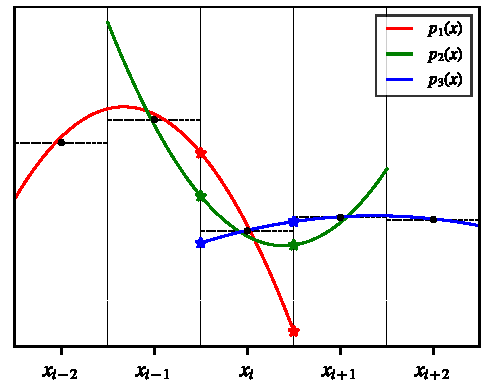
\includegraphics[width=0.85\textwidth]{fig/weno_p1p2p3}
    \caption{The reconstructed profiles in three sub-stencils of the fifth-order WENO-JS scheme.
        The black dots and horizontal dotted lines represent the volume averaged quantities.
        Note that there is a sharp discontinuity at \( x = x_{\imh} \),
        resulting three different reconstructed pointwise values at \( x = x_{i \pm \half} \)
        of each polynomial, marked as stars.
        In ENO perspective, \( p_{3} (x) \) is an appropriate choice, as \( S_{3} = \{ I_{i}, I_{i + 1}, I_{I + 2} \} \)
        does not include the discontinuous point.
    }\label{fig:weno_profiles}
\end{figure}
The core design principle of WENO is to construct nonlinear weights \( \omega_{m} \)
that adaptively select smooth stencils and converges into the linear reconstruction scheme
when all stencils are smooth. Mathematically speaking, the nonlinear weights should
be converged into the \textit{linear weights} \( \gamma_{m}, \; m = 1, 2, 3 \),
\begin{equation}\label{eq:weno_lin_weights}
    \phi (x) = \sum_{m=1}^{3} \gamma_{m} p_{m} (x),
\end{equation}
where \( \phi (x) \) is the reconstructed polynomial within the whole stencil \( S = \bigcup_{m=1}^{3} S_{m} \),
\begin{equation}\label{eq:weno_phi}
    \frac{1}{\dx} \int_{I_{k}} \phi (x) \mathop{dx} = \overline{q}_{k}, \quad
        I_{k} \in \bigcup_{m=1}^{3} S_{m}.
\end{equation}
As the \( \phi (x) \) is the quartic polynomial, it ensures fifth-order convergence rate
of the estimations for pointwise values,
\begin{equation}\label{eq:weno_phi_bigo}
    q_{i \pm \half} = \phi (x_{i \pm \half}) + \mathcal{O}(\dx^{5}).
\end{equation}

Jiang and Shu~\cite{jiang1996efficient} proposed a functional form of
the nonlinear weights by,
\begin{equation}\label{eq:weno_nonlin_weights}
    \omega_{m} = \frac{\widetilde{\omega}_{m}}{\sum_{s} \widetilde{\omega}_{s}}, \quad
        \widetilde{\omega}_{m} = \frac{\gamma_{m}}{{\left( \epsilon + \beta_{m} \right)}^{p}},
\end{equation}
where \( \epsilon \) is the small number (e.g., \( \num{1.E-36} \)) to prevent division by zero,
\( \beta_{m} \) is the smoothness indicator which measures the smoothness of the data
in the given stencil \( S_{m} \).
The parameter \( p \) is an amplification factor for the difference of scales
when a discontinuity is present on one of the candidate stencils.

The remaining step for WENO-JS is to construct the smoothness indicator,
which has large values when the stencil data is not smooth and becomes arbitrary small in a smooth stencil;
thus, it converges to the linear weight.
Jiang and Shu proposed a way to measure the smoothness of the profile based on its second derivatives.
In the fifth-order WENO-JS method, the smoothness indicators \( \beta_{m} \) are given by,
\begin{equation}\label{eq:weno_smoothness_ind}
    \beta_{m} = \sum_{n = 1}^{2} \left( \dx^{2n-1} \int_{I_{i}} {\left[ \frac{d^{n} p_{m} (x)}{dx^{n}} \right]}^{2} \mathop{dx} \right).
\end{equation}

\begin{figure}
    \centering
    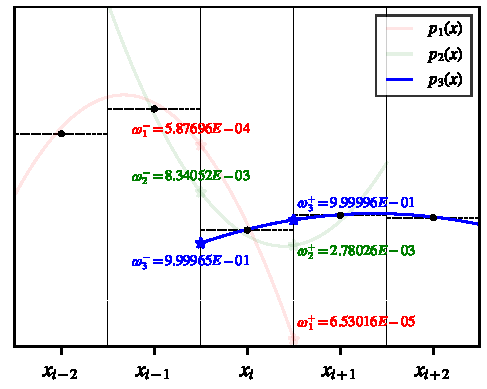
\includegraphics[width=0.85\textwidth]{fig/weno_p1p2p3_nonlinW}
    \caption{The reconstructed fifth-order WENO profiles of the same data stencil in~\cref{fig:weno_profiles},
        combined with WENO-JS nonlinear weights. (\cref{eq:weno_nonlin_weights})
        The opacity of each line measures the nonlinear weights on that sub-stencil,
        and calculated nonlinear weights are noted in the figure.
        Note that the nonlinear weights of \( S_{3} \) are dominant over other stencils, \( S_{1} \) and \( S_{2} \),
        resulting in ENO-style stencil selection.
    }\label{fig:weno_profiles_nonlinW}
\end{figure}

\cref{fig:weno_profiles_nonlinW} shows the effects of the nonlinear weights on the WENO profiles.
The nonlinear weights are calculated through~\cref{eq:weno_nonlin_weights}, with \( p = 2, \; \epsilon = \num{1.E-36} \).
As illustrated in the figure, the nonlinear weights successfully detect the sharp gradient at \( x = x_{\imh} \)
and weighting on \( p_{3} (x) \) dominantly to avoid reconstruction on the discontinuity.



\subsection{Gaussian Process Reconstruction}\label{subsec:gp}

Over decades, the high-order data reconstruction/interpolation methods
for solving hyperbolic PDEs are based on the polynomial approach.
Like the WENO method discussed in the previous section,
the idea starts by assuming a unique polynomial represents the stencil data.
The polynomial-based approaches are the most successful and popular reconstruction/interpolation methods
in the CFD community~\cite{van1979towards,colella1984piecewise,jiang1996efficient,lee2017piecewise}
because of their mathematical simplicity. 

However, the polynomial-based reconstruction/interpolation schemes have some downsides.
Firstly, since the polynomials are not able to represent the discontinuous data,
it is notoriously prone to lead numerical oscillations.
There are several ways to avoid the oscillations, like the WENO method in~\ref{subsec:weno},
but it usually brings complexity and computational expenses.
Another issue for the polynomial-based approach is that the method must be carried out
on a fixed size data stencil, which means changing in stencil size~--~thus it changes the order
of accuracy~--~requires a complete redesign of the code.

Recently, practitioners have designed \textit{non-polynomial} reconstruction/interpolation methods.
Reyes et al.~\cite{reyes2018new,reyes2019variable} proposed a novel way to use the Gaussian process (GP)
to estimate the data at any arbitrary point in high-order accuracy.
Based on the stochastic process, GP reconstruction/interpolation methods are able to predict the data
on desired points (usually at cell interfaces) without considering any polynomials;
therefore, the code is readily extended to a higher order by simply changing the size of the stencil.
In the language of GP, this process can be interpreted in the way that
a probability distribution for the unknown function values \( f(x_{*})\) (pointwise values at arbitrary points \( x_{*} \))
can be trained by the known data \( \overline{q}_{i} \) (volume-averaged quantities at cell centers),
with posterior mean and uncertainty that are compatible with the known observations.

A GP is fully defined by two functions:
\begin{itemize}
    \item a mean function \( \mu_{f} (\bx) = \mathbb{E} \left[ f(\bx) \right] \) over \( \mathbb{R}^{N} \), and
    \item a covariance kernel function, which is symmetric and positive-definite integral kernel
        \( K(\bx, \by) = \mathbb{E}\left[ \left( f(\bx) - \mu_{f} (\bx) \right) \left( f(\by) - \mu_{f} (\by) \right) \right] \)
        over \( \mathbb{R}^{N} \times \mathbb{R}^{N} \),
\end{itemize}
The function \( f \) is then said to belong to the GP with mean and covariance function,
written as \( f \sim GP(\mu_{f} (\bx), K(\bx, \by)) \).

Suppose there are \( N \) sample points for the function \( f \), namely, \( \bff = \left[ f(\bx_{1}), \dots, f(\bx_{N}) \right] \)
that are known, the likelihood \( \mathcal{L} \), the probability of \( \bff \) given the prior GP model,
of the input data \( \bff \), is given by,
\begin{equation}\label{eq:gp_likelihood}
    \mathcal{L} = P(\bff) \equiv \left( 2 \pi \right)^{- \frac{N}{2}} \det \left| \bK \right|^{-\half}
    \exp \left[ -\half \left( \bff - \bmu_{\bff} \right)^{T} \bK \left( \bff - \bmu_{\bff} \right) \right],
\end{equation}
where \( \bK = \left[ K_{ij} \right]_{i, j = 1, \dots, N} \) with \( K_{ij} = K(\bx_{i}, \bx_{j}) \).

The goal of GP is to make a probabilistic statement about the value of \( f_{*} = f (\bx_{*}) \)
of unknown function \( f \sim GP(\mu_{f}, K) \) with given function samples.
By utilizing the conditioning property of GP from the theory of Bayesian inference,
the updated posterior mean function can be obtained as,
\begin{equation}\label{eq:gp_posterior_mean_function}
    \tilde{f}_{*} \equiv \mu_{f}(\bx_{*}) + \bk_{*}^{T} \bK^{-1} \left( \bff - \bmu_{\bff} \right),
\end{equation}
where \( \bk_{*} = \left[ k_{*,i} \right]_{i = 1, \dots, N} \) with \( k_{*,i} = K(\bx_{*}, \bx_{i}) \).
The detailed derivations of \cref{eq:gp_posterior_mean_function} can be found
in the Appendix of~\cite{reyes2018new}.
It is common practice to take the zero mean everywhere, then \cref{eq:gp_posterior_mean_function} becomes
\begin{equation}\label{eq:gp_intp}
    \tilde{f}_{*} = \bk_{*}^{T} \bK^{-1} \bff,
\end{equation}
reveals GP prediction with known function samples \( \bff \), which is the \textit{pointwise} representation.

However, in the reconstruction scheme, the known function samples should be given as \textit{volume averaged} quantities,
not as pointwise values. Therefore, the GP prediction has to be modified to adapt to the data type changes.

Favorably, the volume averaging operator constitutes a linear operation (e.g.,~\cref{eq:recon_poly_linear}).
The linear operations on Gaussian random variables result in new Gaussian random variables with
linearly transformed mean and covariance; thus, the GP \textit{interpolation} scheme (\cref{eq:gp_intp})
can be transformed into the GP \textit{reconstruction} scheme
with proper linear functionals that represent volume-averaging.

Consider a measure \( dg_{k} (\bx) \) on the function \( f(\bx) \) over the cell
\( I_{k} = \prod_{d = x,y,z} I_{k}^{(d)} \) with 1D cells
\( I_{k}^{(d)} = \left[ x_{k}^{(d)} - \frac{\Delta^{(d)}}{2},\; x_{k}^{(d)} + \frac{\Delta^{(d)}}{2} \right] \),
where \( d = x,y,z \) represent the direction of the spatial dimension.
This defines the linear functionals
\begin{equation}\label{eq:gp_vol_intg}
    G_{k} \equiv \int f (\bx) \mathop{d g_{k}(\bx)},
\end{equation}
which represent the volume integral operations on \( f(\bx) \).
The measure \( dg_{k} (\bx) \) are taken to be the cell volume-average measures as,
\begin{equation}\label{eq:gp_dgk}
    dg_{k} (\bx) = \begin{cases}
        d^{3} \bx \cdot \prod\limits_{d = x,y,z} \frac{1}{\Delta^{(d)}} \quad &\text{if } \bx \in I_{k} \\
        0 &\text{otherwise},
    \end{cases}
\end{equation}
where \( \Delta^{(d)} \) is the grid spacing in the \( d \)-direction.
Then, the vector \( \bG \left[ G_{1}, \dots, G_{N} \right]^{T} \)
is normally distributed with mean \( \mathbb{E}(\bG) = \bmu_{\bG} = \left[ \mu_{G_{1}}, \dots, \mu_{G_{N}} \right]^{T} \)
and covariance matrix \( \bC = \left[ C_{kh} \right]_{k,h = 1, \dots, N} \), where
\begin{equation}\label{eq:gp_mu_G}
    \mu_{G_{k}} = \mathbb{E} [G_{k}] = \int \mathbb{E} \left[ f(\bx) \right] \mathop{d g_{k} (\bx)} = \int \mu_{f} (\bx) \mathop{d g_{k} (\bx)},
\end{equation}
and
\begin{equation}\label{eq:gp_Ckh}
    \begin{split}
        C_{kh} &= \mathbb{E} \left[ \left( G_{k} - \mu_{G_{k}} \right) \left( G_{h} - \mu_{G_{h}} \right) \right] \\
               &= \int \int \mathbb{E} \left[ \left( f(\bx) - \mu_{f} (\bx) \right) \left( f(\by) - \mu_{f} (\by) \right)\right] \mathop{d g_{k}(\bx)} \mathop{d g_{h} (\by)} \\
               &= \int \int K (\bx, \by) \mathop{d g_{k} (\bx)} \mathop{d g_{h} (\by)}.
    \end{split}
\end{equation}
Thus, the GP distribution on the function \( f \sim GP(\mu, K) \) conducts a multivariate
Gaussian distribution on \( N \)-dimensional vector \( \bG \) of linear functionals of \( f \).

In order to generalize~\cref{eq:gp_intp} for reconstruction, the remaining task is to define
the prediction vector \( \bT_{*} = \left[ \bT_{*,k} \right]_{k = 1, \dots, N} \)
at any arbitrary point of interest \( \bx_{*} \) as,
\begin{equation}\label{eq:gp_pred_vec}
    \begin{split}
        T_{*, k} &= \mathbb{E} \left[ \left( f(\bx_{*}) - \mu_{f}(\bx_{*}) \right) \left( G_{k} - \mu_{G_{k}} \right) \right] \\
                 &= \int K (\bx_{*}, \bx) \mathop{d g_{k} (\bx)}.
    \end{split}
\end{equation}
Finally, the pointwise estimation of \( f(\bx_{*}) \) at the point of \( \bx_{*} \),
reconstructed from the volume-averaged data \( \bG \) is given by,
\begin{equation}\label{eq:gp_recon}
    \tilde{f}_{*} = \bT_{*}^{T} \bC^{-1} \bG,
\end{equation}
with zero mean values. \cref{eq:gp_recon} shows the explicit form of GP reconstruction
with known volume-averaged data points, \( \bG \). The terms \( \bC \) and \( \bT \) are determined by
the choice of the covariance kernel function, \( K(\bx, \by) \), which measures the relationship between pairs of data.
In this dissertation, the ``Squared Exponential'' (SE) kernel used for GP reconstruction.
\begin{equation}\label{eq:gp_se_kernel}
    K_{\text{SE}} (\bx, \by) = \Sigma^{2} \exp \left[ -\frac{\left( \bx - \by \right)^{2}}{2 \ell^{2}} \right].
\end{equation}
The SE kernel has two hyperparameters \( \Sigma \) and \( \ell \),
but the hyperparameter \( \Sigma \) has no effect on the posterior mean function,
so this dissertation set \( \Sigma = 1 \) for simplicity.
On the other hand, the hyperparameter \( \ell \) expresses the correlation length scale of the model,
so it should be chosen meticulously corresponding to the physical length scale of the grid configuration.

For 1D reconstructions, \( T_{*, k} \) and \( C_{kh} \) for SE kernel becomes,
\begin{equation}\label{eq:gp_se_T}
    T_{*,k} = \sqrt{\frac{\pi}{2}}\frac{\ell}{\Delta} \left \{
        \erf{\frac{\Delta_{k*}+1/2}{\sqrt{2}\ell/\Delta}}
        - \erf{\frac{\Delta_{k*}-1/2}{\sqrt{2}\ell/\Delta}}
     \right \},
\end{equation}
and
\begin{equation}\label{eq:gp_se_C}
    \begin{split}
        C_{kh} = \sqrt{\pi} & \left( \frac{\ell}{\Delta} \right)^{2}
        \left \{
            \left( \frac{\Delta_{kh} + 1}{\sqrt{2} \ell / \Delta} \erf{\frac{\Delta_{kh} + 1}{\sqrt{2} \ell / \Delta}} +
                \frac{\Delta_{kh} - 1}{\sqrt{2} \ell / \Delta} \erf{\frac{\Delta_{kh} - 1}{\sqrt{2} \ell / \Delta}}
            \right) \right. \\
            &+ \frac{1}{\sqrt{\pi}} \left(
                \exp \left[ - \frac{\left( \Delta_{kh} + 1 \right)^{2}}{2 \left( \ell / \Delta \right)^{2}} \right]
                + \exp \left[ - \frac{\left( \Delta_{kh} -1 \right)^{2}}{2 \left( \ell / \Delta \right)^{2}} \right]
            \right) \\
            &\left.
            -2 \left(
                \frac{\Delta_{kh}}{\sqrt{2} \ell / \Delta} \erf{\frac{\Delta_{kh}}{\sqrt{2} \ell / \Delta}}
                + \frac{1}{\sqrt{\pi}} \exp \left[ -\frac{\Delta_{kh}^{2}}{2 \left( \ell / \Delta \right)^{2}} \right] 
            \right)
        \right \},
    \end{split}
\end{equation}
where \( \Delta_{kh} = (x_{k} - x_{h})/\Delta \) and \( \Delta \) is the grid spacing along the 1D direction.
Note that the analytic derivations of \( T_{*, k} \) and \( C_{kh} \) above
only depend on the grid spacing and the length between the prediction point \( \bx_{*} \)
and the locations of known training data. With uniform grid configuration,
those values are established at the initial step.
Since the prediction points are the cell interfaces \( x_{i \pm \half} \)
for the conventional FDM constructions, one can save,
\begin{equation}\label{eq:gp_zvec}
    \bz_{i \pm \half} \coloneqq \bT^{T}_{i \pm \half} \bC^{-1},
\end{equation}
as the weighting factor for the reconstruction can be expressed as,
\begin{equation}\label{eq:gp_recon_with_zvec}
    q_{i \pm \half} = \bz^{T}_{i \pm \half} \bG,
\end{equation}
for computational efficiency.

\begin{figure}
    \centering
    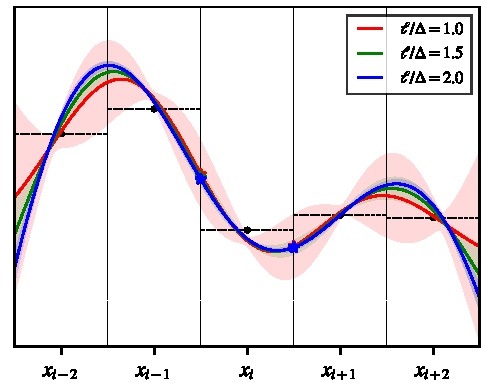
\includegraphics[width=0.85\textwidth]{fig/gp_linear_recon}
    \caption{GP reconstructed profiles with the same data as~\cref{fig:weno_profiles,fig:weno_profiles_nonlinW}
        with different hyperparameters \( \ell = 1.0, 1.5, 3.0 \).
        Note that all the reconstructed profiles produce a new local minimum near \( x = x_{\iph} \),
        which violates the monotonic-preserving condition and leads to numerical oscillations.
        The shaded areas represent 95\% confidence regions from the posterior variance.
    }\label{fig:gp_linear_recon}
\end{figure}

However, the GP reconstruction also needs special handling for the discontinuous profiles,
like the nonlinear weightings in the WENO method in~\cref{subsec:weno}.
\cref{fig:gp_linear_recon} shows the GP reconstructions with the same data as~\cref{fig:weno_profiles,fig:weno_profiles_nonlinW},
with \( \ell = 1, 1.5, 3 \). The initial profile has a strong gradient at \( x = x_{\imh} \);
hence, the GP reconstructed profiles have undershot values at \( x = x_{\iph} \).

Reyes et al.~\cite{reyes2019variable} proposed a WENO-\textit{like} approach to
the GP reconstruction/interpolations by considering the GP marginal likelihood of the local stencil data
for measuring the smoothness of the stencil,
and use them to construct nonlinear weights as like in the standard WENO method.

For five points, fifth-order GP reconstruction, suppose three sub-stencils as like fifth-order WENO method. (\cref{eq:weno_substencils})
Then there are three reconstructed pointwise values for each of the candidate stencils \( S_{m} \),
\begin{equation}\label{eq:gp_weno_candidates}
    q_{i \pm \half, m} = \bz_{i \pm \half, m}^{T} \bG_{m}.
\end{equation}
The final reconstructed value is taken as the combinations of three candidate GP approximations with nonlinear weights,
\begin{equation}\label{eq:gp_weno_comb}
    q_{i \pm \half} = \sum_{m = 1}^{3} \omega_{m} q_{i \pm \half, m}.
\end{equation}

As in the conventional WENO method, the nonlinear weights \( \omega_{m} \)
must be reduced to the optimal (linear) weights \( \gamma_{m} \) in a smooth region,
so the weighted combination~\cref{eq:gp_weno_comb} converges to the GP approximation
over the whole stencil \( S = \bigcup_{m} S_{m} \). The optimal weights \( \gamma_{m} \) must satisfy,
\begin{equation}\label{eq:gp_weno_linW}
    \bz_{i \pm \half}^{T} \bG = q_{i \pm \half} = \sum_{m=1}^{3} \gamma_{m} q_{i \pm \half, m} = \sum_{m=1}^{3} \gamma_{m} \bz_{i \pm \half, m}^{T} \bG_{m},
\end{equation}
or explicitly,
\begin{equation}\label{eq:gp_weno_overdetermined}
    \gamma_{1}
    \left[
        \begin{array}{c}
            \mathrm{z}_{1,1}^{\pm} \\
            \mathrm{z}_{2,1}^{\pm} \\
            \mathrm{z}_{3,1}^{\pm} \\
            0 \\
            0 \\
        \end{array}
    \right]
    \hspace{-30.0\arrayrulewidth}
    \begin{array}[c]{@{}l@{\,}l}
       \left.
       \begin{array}{c}
           \vphantom{\vdots}\\
           \vphantom{0}
       \end{array}
       \right\}
       &
       {\bz_{i \pm \half, 1}} \\ \\ \\
    \end{array}
    \hspace{-20.0\arrayrulewidth}
+
    \gamma_{2}
    \left[
        \begin{array}{c}
            0 \\
            \mathrm{z}_{1,2}^{\pm} \\
            \mathrm{z}_{2,2}^{\pm} \\
            \mathrm{z}_{3,2}^{\pm} \\
            0 \\
        \end{array}
    \right]
    \hspace{-30.0\arrayrulewidth}
    \begin{array}[c]{@{}l@{\,}l}
       \left.
       \begin{array}{c}
           \vphantom{\vdots}\\
           \vphantom{0}
       \end{array}
       \right\}
       &
       {\bz_{i \pm \half, 2}} \\
    \end{array}
    \hspace{-20.0\arrayrulewidth}
+
    \gamma_{3}
    \left[
        \begin{array}{c}
            0 \\
            0 \\
            \mathrm{z}_{1,3}^{\pm} \\
            \mathrm{z}_{2,3}^{\pm} \\
            \mathrm{z}_{3,3}^{\pm} \\
        \end{array}
    \right]
    \hspace{-30.0\arrayrulewidth}
    \begin{array}[c]{@{}l@{\,}l} \\ \\
       \left.
       \begin{array}{c}
           \vphantom{\vdots}\\
           \vphantom{0}
       \end{array}
       \right\}
       &
       {\bz_{i \pm \half, 3}}
    \end{array}
    \hspace{-20.0\arrayrulewidth}
=
    \left[
        \begin{array}{c}
            \mathrm{z}_{1}^{\pm} \\
            \mathrm{z}_{2}^{\pm} \\
            \mathrm{z}_{3}^{\pm} \\
            \mathrm{z}_{4}^{\pm} \\
            \mathrm{z}_{5}^{\pm} \\
        \end{array}
    \right]
    \hspace{-30.0\arrayrulewidth}
    \begin{array}[c]{@{}l@{\,}l}
       \left.
       \begin{array}{c}
           \vphantom{0} \\
           \vphantom{\vdots} \\
           \vphantom{\vdots} \\
           \vphantom{0}
           \end{array}
       \right\}
       &
       \bz_{i \pm \half} \\
    \end{array}.
\end{equation}
The \cref{eq:gp_weno_overdetermined} can be rewritten in the matrix form
of overdetermined system as,
\begin{equation}\label{eq:gp_weno_overdetermined_matrix}
    \left[ 
        \begin{array}{ccc}
            {\mathrm{z}_{1,1}^{\pm}}  & 0                       & 0 \\
            {\mathrm{z}_{2,1}^{\pm}}  & \mathrm{z}_{1,2}^{\pm}  & 0 \\
            {\mathrm{z}_{3,1}^{\pm}}  & \mathrm{z}_{2,2}^{\pm}  & \mathrm{z}_{1,3}^{\pm} \\
            0                         & \mathrm{z}_{3,2}^{\pm}  & \mathrm{z}_{2,3}^{\pm} \\
            0                         & 0                       & \mathrm{z}_{3,3}^{\pm} \\
        \end{array}
    \right]
%
\left[
    \begin{array}{c}
        \gamma_1\\
        \gamma_2\\
        \gamma_3\\
    \end{array}
\right]
%
=
%
\left[
    \begin{array}{c}
        {\mathrm{z}_{1}^{\pm}} \\
        {\mathrm{z}_{2}^{\pm}} \\
        {\mathrm{z}_{3}^{\pm}} \\
        {\mathrm{z}_{4}^{\pm}} \\
        {\mathrm{z}_{5}^{\pm}} \\
    \end{array}
\right].
\end{equation}
Thus, the optimal weights \( \gamma_{m}, m = 1, 2, 3 \) are obtained by solving the overdetermined system,
\cref{eq:gp_weno_overdetermined_matrix}. It should be noted that the optimal weights are
entirely determined by the choice of kernel function and the stencil size,
so they are computed and stored before the simulation begins.

For constructing WENO nonlinear weights~\cref{eq:weno_nonlin_weights},
the only remaining task is to determine the smoothness indicator, \( \beta_{m} \),
which measures the degree of smoothness of a given stencil of data.
Unlike the conventional WENO method, which measures the smoothness of the data
by calculating \( L_{2} \) norms of all the derivatives of the reconstructed polynomials,
the GP reconstruction method should take a different approach to specify the smoothness indicator
because there is no polynomial defined in GP\@.
One successful practice is to use the marginal likelihood of the data.
The likelihood function is well-furnished to gauge the deviations from smoothness
given a sufficiently smooth covariance kernel function, SE kernel, for example.
Thus, the GP predictions have smaller likelihoods to non-smooth function by its design.

Suppose the negative log of the GP marginal likelihood as
\begin{equation}\label{eq:gp_log_marginal_likelihood}
    -\log \mathcal{L} = \frac{N}{2} \log \left[ 2 \pi \right] + \half \log \left| \det \bK_{m} \right|
        + \half \left( \bff_{m} - \bmu_{\bff} \right)^{T} \bK_{m}^{-1} \left( \bff_{m} - \bmu_{\bff} \right),
\end{equation}
then the three terms on the right-hand side of~\cref{eq:gp_log_marginal_likelihood} are revealed as
a normalization, a complexity penalty, and a data fit term, respectively.
The normalization term and the complexity penalty have no effects on defining smoothness indicators
in a uniform grid configuration; only the data fit term along with the choice of zero mean is used
for constructing smoothness indicators in GP,
\begin{equation}\label{eq:gp_smoothness_ind}
    \beta_{m} = \bff_{m}^{T} \left( \bK^{-1}_{m} \right) \bff_{m}.
\end{equation}
To handle discontinuity, a second hyperparameter, \( \sigma \), should be used in~\cref{eq:gp_smoothness_ind},
to discriminate discontinuities from smooth regions. \( \sigma \) should be on the order of the grid spacing.

Like GP reconstruction weights~\cref{eq:gp_recon_with_zvec}, the calculations of
GP smoothness indicators \( \beta_{m} \) can be expressed in a more computationally efficient form.
Considering the eigensystem \( \bK_{m}^{-1} = \sum_{i} \mathbf{v}_{i}^{m} \left( \mathbf{v}_{i}^{m} \right)^{T}/\lambda_{i}^{m} \),
\begin{equation}\label{eq:gp_smoothness_ind_with_eig}
    \beta_{m} = \sum_{i=1}^{3} \bff_{m}^{T} \left( \frac{\mathbf{v}_{i}^{m} \left( \mathbf{v}_{i}^{m} \right)^{T}}{\lambda_{i}} \right) \bff_{m},
\end{equation}
in the five-point, three-stencil GP-WENO method\@.
Again, the observed (training) data is in the volume-averaged form;
thus, the data-type conversion should be examined:
\begin{equation}\label{}
    \bff_{m} = \mathbf{Z}_{m}^{T} \bG_{m},
\end{equation}
where each column vector of \( \mathbf{Z}_{m} \) is given by the GP reconstructing weight, \( \bz \), (see~\cref{eq:gp_zvec})
for each elements of \( \bff_{m} \).

Lastly, the calculation of the smoothness indicator beta can be expressed in the compact form as,
\begin{equation}\label{eq:gp_weno_smooth_ind}
    \begin{split}
        \beta_{m} &= \sum_{i=1}^{3} \left( \frac{ \left( \mathbf{v}_{i}^{m} \right)^{T} \mathbf{Z}_{m}^{T} \bG_{m} }{\sqrt{\lambda_{i}^{m}}} \right)^{2} \\
                  &= \sum_{i=1}^{3} \left( \bP_{i}^{m} \bG_{m} \right)^{2},
    \end{split}
\end{equation}
where \( \bP_{i}^{m} \coloneqq \frac{ \left(\mathbf{v}_{i}^{m}\right)^{T} \mathbf{Z}_{m}^{T}}{\sqrt{\lambda_{i}^{m}}} \),
which can be established before the simulation start, in uniform grid configuration.

Now, the nonlinear weights for GP-WENO reconstruction are fully determined
with~\cref{eq:weno_nonlin_weights}.
In the stepwise representation, the GP-WENO reconstruction scheme for FDM formulation
in the unifrom grid can be summarized as below:
\begin{enumerate}
    \item Before the simulation starts, calculate the following values and store them for later reconstructions:
        \begin{enumerate}
            \item Reconstruction weights, \( \bz_{m} \) (\cref{eq:gp_weno_candidates}) for each candidate stencil, \( m \).
            \item Linear weights, \( \gamma_{m} \), by the solving overdetermined system, \cref{eq:gp_weno_overdetermined_matrix},
                using the least square method.
            \item \( \bP_{i}^{m} \) (\cref{eq:gp_weno_smooth_ind}) for calculating smoothness indicator \( \beta_{m} \) in later.
        \end{enumerate}
    \item During the simulation, at each reconstruction step of cell \( I_{i} \):
        \begin{enumerate}
            \item Calculate nonlinear weights, \( \omega_{m} \), following the conventional WENO method. (\cref{eq:weno_nonlin_weights})
            \item Compute \( m \)-number of reconstructed candidate data, \( q_{i \pm \half, m} \). (\cref{eq:gp_weno_candidates})
            \item Taking weighted combinations of \( q_{i \pm \half, m} \), with nonlinear weights, \( \omega_{m} \),
                and finalize the reconstruction step at \( x_{i} = x_{i \pm \half} \). (\cref{eq:gp_weno_comb})
        \end{enumerate}
\end{enumerate}

\begin{figure}
    \centering
    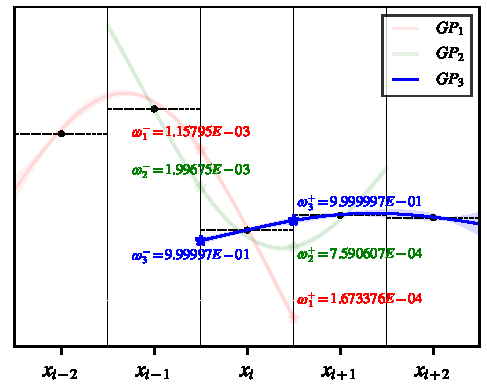
\includegraphics[width=0.85\textwidth]{fig/gp_weno_nonlinW}
    \caption{GP-WENO Reconstructed profiles with nonlinear weights with the same data as~\cref{fig:gp_linear_recon}.
        Hyperparameters \( \ell = 2\Delta \) and \( \sigma = 2\Delta \) are used. 95\% confidence regions
        are shaded with the correspoinding colors, and the opacity of each prediction measures the nonlinear weights
        on that sub-stencil.
    }\label{fig:gp_weno_nonlinW}
\end{figure}




\section{High-Order Time Integration Schemes}\label{sec:time_integration}

A high-order temporal discretization scheme ought to be considered alongside
the high-order spatial data interpolation/reconstruction to acquire
highly accurate numerical solutions in FDM formulation.
The numerical errors arise from both spatial and temporal discretizations
since the solution of the conservative PDEs lies on the spatio-temporal plane.
The overall order of solution accuracy will be determined by the highest order term
of the truncation errors both from the spatial and temporal discretization, i.e.,
\( \mathcal{O}(\Delta s^{p}, \Delta t^{q}) \).
For example, if the leading error term from the temporal discretization
is significantly larger than the leading error term from the spatial discretizations,
\( \mathcal{O}(\dt^{q}) > \mathcal{O}(\Delta s^{p}) \),
then the solution accuracy will be degraded by order of temporal accuracy, \( q \),
no matter the order of spatial accuracy is used.
Therefore, a high-order FDM scheme requires a meticulously designed
temporal discretization method that ensures the solution’s accuracy and stability.

\subsection{Strong Stability Preserving Runge-Kutta Methods}\label{subsec:ssprk}

The Runge-Kutta (RK) method is the most popular way to integrate
the semi-discretized form of FDM (\cref{eq:fdm_discrete}) over the time axis.
The key idea is to treat the~\cref{eq:fdm_discrete} as an ordinary differential equation (ODE)
at each lattice point on the computational mesh as,
\begin{equation}\label{eq:fdm_mol}
    \pd{\bU_{i}}{t} = \mathcal{L}_{i} (\bU),
\end{equation}
where the right-hand side operator \( \mathcal{L}_{i} \) is given by the spatial discretization method at cell \( I_{i} \).
The RK approach can be viewed as a strategy to integrate PDEs by solving several ODE problems at each discretized time domain.
In general, \( m \)-stage RK method which integrate~\cref{eq:fdm_mol}
from \( t = t^{n} \) to \( t = t^{n} + \dt = t^{n + 1} \) is given by,
\begin{equation}\label{eq:general_rk}
    \begin{split}
        \bU^{(0)} &= \bU^{n}, \\
        \bU^{(l)} &= \sum_{k=0}^{l -1} \left( \alpha_{l, k} \bU^{(k)} + \dt \beta_{l,k} \mathcal{L} (\bU^{(k)}) \right), \quad \alpha_{l,k} \geq 0, \quad l = 1, \dots, m \\
        \bU^{n + 1} &= \bU^{(m)},
    \end{split}
\end{equation}
where the spatial discretization index, \( i \), is omitted for simplicity.
Therefore, the coefficients \( \alpha_{l,k} \) and \( \beta_{l,k} \) fully determine
the numerical accuracy and stability of the RK scheme.

Like the spatial discretization method, it is crucial to consider the TVD property of the temporal discretization scheme.
Gottlieb and her collaborators~\cite{gottlieb1998total,gottlieb2001strong,gottlieb2011strong}
developed the so-called strong stability preserving Runge-Kutta (SSP-RK) method,
which ensures TVD property by sequentially applying convex combinations of the
first-order forward Euler method as a building-block at each sub-stage.
In this way, the desired TVD property is achieved if each of the sub-stage is TVD\@.

SSP-RK method uses that the forward Euler method for building each sub-stages.
Since the forward Euler method is strongly stable under the Courant–Friedrichs–Lewy (CFL) condition;
thus, if all sub-stages of the RK method can be described as a form of the forward Euler method,
then the TVD property is fulfilled by virtue of the forward Euler method.
It is easy to see in~\cref{eq:general_rk} that the sub-stages of the RK method, \( \bU^{(l)} \)
can be described as the forward Euler method if all the \( \beta_{l, k} \) are nonnegative \( \beta_{l, k} \geq 0 \)
by replacing \( \dt \) by \( \frac{\beta_{l, k}}{\alpha_{l, k}} \dt \).
For example, in~\cite{gottlieb1998total}, Gottlieb found the optimal third-order
SSP-RK method given by,
\begin{equation}\label{eq:ssp_rk3}
    \begin{split}
        \bU^{(1)} &= \bU^{n} + \dt \mathcal{L}(\bU^{n}), \\
        \bU^{(2)} &= \frac{3}{4} \bU^{n} + \frac{1}{4} \bU^{(1)} + \frac{1}{4} \dt \mathcal{L}(\bU^{(1)}), \\
        \bU^{n + 1} &= \frac{1}{3} \bU^{n} + \frac{2}{3} \bU^{(2)} + \frac{2}{3} \dt \mathcal{L}(\bU^{(2)}),
    \end{split}
\end{equation}
which requires three sub-stages for integrating from \( t = t^{n} \) to \( t = t^{n + 1} \).

The above third-order, three-stages SSP-RK method~\cref{eq:ssp_rk3} is by far
the most famous high-order time integrator used in most high-order method researches in the CFD community.
In practice, spatial accuracy is often considered to carry more weight than temporal accuracy
in designing higher accurate spatial models~\cite{balsara2000monotonicity,mignone2010high},
so combining the high-order spatial method (generally, fifth-order or higher)
with a relatively low-order temporal scheme (third-order SSP-RK) could be justifiable.
However, as it is shown in~\cite{lee2021recursive}, the order of convergence rate of the solution
can be degraded by the order of temporal method (e.g., third-order) in high-resolution computational grids,
so using a higher than third-order temporal scheme is required for maintaining desired spatial accuracy in a high-resolution grid.

In contrast to the third-order SSP-RK3 method, devising a fourth-order SSP-RK4
is more involved to meet the favorable SSP property, which is ensured by positive coefficients.
Several theoretical studies have shown that a fourth-order SSP-RK4
cannot be formulated with just four sub-stages and positive coefficients~\cite{gottlieb1998total},
meaning that the classical four-stage, fourth-order RK is not SSP\@.
For example, by far the most optimal fourth-order, fourth-stage SSP-RK method is:
\begin{equation}\label{eq:ssp_rk44_negatives}
    \begin{split}
        \bU^{(1)} &= \bU^{n} + \half \dt \mathcal{L}(\bU^{n}), \\
        \bU^{(2)} &= \frac{649}{1600} \bU^{(0)} - \frac{10890423}{25193600} \dt \tilde{\mathcal{L}} (\bU^{n}) + \frac{951}{1600} \bU^{(1)} + \frac{5000}{7873} \dt \mathcal{L}(\bU^{(1)}), \\
        \bU^{(3)} &= \frac{53989}{2500000} \bU^{n} - \frac{102261}{5000000} \dt \tilde{\mathcal{L}} (\bU^{n}) + \frac{4806213}{20000000} \bU^{(1)} \\
            &\quad - \frac{5121}{20000} \dt \tilde{\mathcal{L}}(\bU^{(1)}) + \frac{23619}{32000} \bU^{(2)} + \frac{7873}{10000} \dt \mathcal{L}(\bU^{(2)}), \\
        \bU^{(4)} &= \frac{1}{5} \bU^{n} + \frac{1}{10} \dt \mathcal{L}(\bU^{n}) + \frac{6127}{30000} \bU^{(1)} + \frac{1}{6} \dt \mathcal{L}(\bU^{(1)}) + \frac{7873}{30000} \bU^{(2)} \\
            &\quad + \frac{1}{3} \bU^{(3)} + \frac{1}{6} \dt \mathcal{L}(\bU^{(3)}).
    \end{split}
\end{equation}
Note that the above four-stage, fourth-order SSP-RK method uses the adjoint spatial operator, \( \tilde{\mathcal{L}} \),
to bear the negative coefficients, e.g., \( -\frac{10890423}{25193600} \) and \( -\frac{102261}{5000000} \).
Numerically speaking, the only difference between \( \mathcal{L} \) and \( \tilde{\mathcal{L}} \)
is the direction of the upwind limiting. Although the computational cost of calculating \( \mathcal{L}(\bU) \) and
\( \tilde{\mathcal{L}}(\bU) \) are identical, but it demands separated codes, and leads implementation complexity.

Spiteri and Ruuth~\cite{spiteri2002new} proposed a five-stage, fourth-order SSP-RK4 method that does not require to use adjoint operator:
\begin{equation}\label{eq:ssp_rk4}
\resizebox{1.0\textwidth}{!}
    {$\begin{split}
        \bU^{(1)} &= \bU^{n} + 0.391752226571890 \dt \mathcal{L}(\bU^{n}), \\
        \bU^{(2)} &= 0.444370493651235 \bU^{n} + 0.555629506348765 \bU^{(1)} + 0.368410593050371 \dt \mathcal{L} (\bU^{(1)}), \\
        \bU^{(3)} &= 0.620101851488403 \bU^{n} + 0.379898148511597 \bU^{(2)} + 0.251891774271694 \dt \mathcal{L} (\bU^{(2)}), \\
        \bU^{(4)} &= 0.178079954393132 \bU^{n} + 0.821920045606868 \bU^{(3)} + 0.544974750228521 \dt \mathcal{L} (\bU^{(3)}), \\
        \bU^{n + 1} &= 0.517231671970585 \bU^{(2)} + 0.096059710526147 \bU^{(3)} + 0.063692468666290 \dt \mathcal{L} (\bU^{(3)}) \\
                    &\quad + 0.386708617503268 \bU^{(4)} + 0.226007483236906 \dt \mathcal{L} (\bU^{(4)}).
    \end{split}$}
\end{equation}
In this dissertation, the fourth-order SSP-RK4 method refers the Spiteri and Ruuth method,~\cref{eq:ssp_rk4}.

In many studies about high-order CFD solvers~\cite{gottlieb1998total,gottlieb2001strong,gottlieb2011strong,mignone2010high,del2003efficient,del2007echo,reyes2018new,reyes2019variable},
the SSP-RK schemes have proven high fidelity and portability, guaranteeing high-order accuracy
and numerical stability with TVD property.
However, the very nature of the SSP-RK method~-- being a multi-stage approach --~increases
computational costs in CFD simulations.
In SSP-RK methods, the data reconstruction/interpolation (i.e., \( \mathcal{L}(\cdot) \)) and the boundary condition
should be applied in each sub-stage, which increases the computational resources
and the footprint of data communications in the parallel computational architecture.
It makes the simulations using the adaptive mesh refinement (AMR) method less attractive,
which progressively refines the grid resolutions
and increases data communications around the simulations’ interesting features.


\subsection{Lax–Wendroff Type Methods}\label{subsec:laxwendroff}

The Lax-Wendroff method~\cite{lax1959systems} rely on the Taylor expansion in time
to achieve high-order in time accuracy:
\begin{equation}\label{eq:lw_time_taylor}
    \bU^{n + 1} = \bU^{n} + \dt \left. \pd{\bU}{t} \right|^{n} + \frac{\dt^{2}}{2!} \left.\pdd{\bU}{t}\right|^{n} + \mathcal{O}(\dt^{3}).
\end{equation}
The temporal derivatives can be transformed into spatial derivatives
by applying the Lax-Wendroff or Cauchy-Kowalewski procedure (LW/CK hereafter).
In one-dimensional conservative PDEs, for example,
\begin{equation}\label{eq:lw_1d_ck_procedure}
    \begin{split}
        \pd{\bU}{t} &= -\pd{\bF}{x}, \\
        \pdd{\bU}{t} &= \pd{}{t} \left( -\pd{\bF}{x}\right) \\
                     &= -\pd{}{x} \left( \pd{\bF}{\bU} \cdot \pd{\bU}{t} \right) \\
                     &= \pd{}{x} \left( \pd{\bF}{\bU} \cdot \pd{\bF}{x} \right),
    \end{split}
\end{equation}
where \( \pd{\bF}{\bU} \) is a flux Jacobian matrix.
In the original Lax-Wendroff method~\cite{lax1959systems} used an approximation of \( \pd{}{x} \left( \pd{\bF}{\bU} \cdot \pd{\bF}{x} \right) \approx
\frac{1}{\dx}\left( \left.\pd{\bF}{\bU} \right|_{\iph} \cdot \pd{\bF}{x} - \left.\pd{\bF}{\bU} \right|_{\imh} \cdot \pd{\bF}{x} \right) \),
but it is possible to get an explicit form as,
\begin{equation}\label{}
    \pdd{\bU}{t} = \pd{}{x} \left( \pd{\bF}{\bU} \cdot \pd{\bF}{x} \right) = \pdd{\bF}{\bU} \cdot \pd{\bF}{x} + \pd{\bF}{\bU} \cdot \pdd{\bF}{x},
\end{equation}
with flux Hessian tensor, \( \pdd{\bF}{\bU} \).

The primary advantage of the Lax-Wendroff method is that
it can achieve a high order in time accuracy within a single step of the calculation.
The idea to construct the time-Taylor series by harnessing the tight coupling of temporal
and spatial derivatives through LW/CK procedures inspires many practitioners
to develop single-step, high-order methods based on the Lax-Wendroff method.

In 2001, Toro et al.~\cite{toro2001towards} extended this idea
by combining it with the generalized Riemann problems (GRPs)
and introduced the Arbitrary high order derivative Riemann problem (ADER) method.
Toro and his collaborators constructed Riemann problems for each spatial derivative at cell interface, \( x_{\iph} \):
\begin{equation}\label{eq:toro_ader_dudx}
    \begin{split}
        &\pd{\bU^{(k)}_{x}}{t} + \left. \pd{\bF}{\bU} \right|_{\iph} \pd{\bU^{(k)}_{x}}{x} = 0, \quad \text{where } \left. \pd{\bF}{\bU} \right|_{\iph} = \pd{\bF}{\bU}(\bU_{\iph}, 0^{+}), \\
        &\bU^{(k)}_{x} (x, 0) =
        \begin{cases}
            \frac{\partial^{k}}{\partial x^{k}} \bU_{\iph, L}, \quad x < x_{\iph}, \\
            \frac{\partial^{k}}{\partial x^{k}} \bU_{\iph, R}, \quad x > x_{\iph},
        \end{cases}
    \end{split}
\end{equation}
where \( \bU^{(k)}_{x} = \frac{\partial^{k} \bU}{\partial x^{k}} \), and
\( \bU_{\iph, LR} \) represent left and right Riemann states at cell interface, \( x_{\iph} \).
Reconstructed profiles can find the Riemann states of the spatial derivatives.
The resulting solutions of the above Riemann problems
are then applied for LW/CK procedures to get the temporal derivatives, \( \left. \frac{\partial^{k} \bU}{\partial t^{k}} \right|_{\iph} \),
and they are used to construct the time-Taylor series of the conservative variables at cell interfaces:
\begin{equation}\label{eq:toro_ader}
    \bU (x_{\iph}, \tau) = \bU(x_{\iph}, 0^{+}) + \sum_{k = 1}^{r -1} \left[ \frac{\partial^{k}}{\partial t^{k}} \bU (x, t) (x_{\iph}, 0^{+}) \right] \frac{\tau^{k}}{k!}.
\end{equation}
% Toro and his collaborators applied LW/CK procedures
% to get the coefficients of the power series expansion of the conservative variables
% and solved GRPs for each high-order term.
% For instance, Toro considered a time-Taylor series of conservative variables
% at cell interface, \( \bU_{\iph} \), in arbitrary order as,

ADER methods were further developed in~\cite{toro2001towards,titarev2002ader,titarev2005ader},
and it has grown its popularity over decades,
leading to various further modifications.
ADER-DG~\cite{fambri2017space,zanotti2016efficient} and
ADER-CG~\cite{balsara2009efficient,balsara2013efficient,balsara2017higher}
in the context of discontinuous and continuous Galerkin schemes;
other efforts of employing
an implicit GRP solver
to solve  scalar equations 
with stiff source terms~\cite{montecinos2012solver},
its extensions to second-order schemes for 
nonlinear systems~\cite{montecinos2014reformulations}
and to general hyperbolic systems~\cite{toro2015implicit}.
The use of an implicit time Taylor series expansion for GRP
was further simplified
in the study by Montecinos and Balsara~\cite{montecinos2020simplified}.
Along the line of simplifying the standard ADER approach,
the Differential Transform Method (DTM)~\cite{chen1996application}
was also adopted to alleviate
the cost of the ADER scheme, coined as ADER-DT (or ADER-Taylor)
in~\cite{norman2012multi,norman2013algorithmic,norman2014weno}.

In general, Lax-Wendroff type methods are able to update the solution
in single-step with high-order temporal accuracy.
The fundamental advantage of being a single-stage method is the enhanced performance.
This becomes hugely attractive in massively parallel computing, minimizing the computational frequency
of data transfers between processors each time step, which would need to be repeated for each intermediate RK stage.
On the other hand, the dependence of the strong coupling on analytic derivatives
of the governing PDEs makes the LW/CK approach less flexible and less broadly applicable to all systems of PDEs.





\section{Conclusion}\label{sec:high_order_conclusion}

The high-order discretization methods promote better solution accuracy in the given grid resolutions.
In order to achieve high-order accuracy of the conservative system,
high-arithmetic-intensity numerical models should be accomplished
both in spatial and temporal axes.

Under the finite difference formulation,
the high-order reconstruction methods play a role in discretizing the spatial axis
with better solution accuracy by estimating the pointwise data with given volume-averaged quantities.
The high-order reconstruction schemes for CFD solvers are also required to have TVD property
to reduce the numerical oscillations near the discontinuous profiles.
The general strategy is to reduce the order of accuracy locally where the given profile is discontinuous.
The conventional WENO method constructs
the piecewise polynomials by taking the convex combinations of sub-polynomials with nonlinear weightings.

The WENO method
\begin{itemize}
    \item achieves high-order accuracy by constructing the piecewise polynomials, and
    \item measures the smoothness of the given data by calculating spatial derivatives of the reconstructed profiles.
\end{itemize}

GP-WENO method is another class of non-polynomial-based reconstruction strategy
utilizing the Gaussian Process.
The GP reconstruction is based on the conventional GP regression scheme,
with modifications of the kernel function
to adopt the data type conversion from volume-averaged to pointwise.
The GP method provides a more compact mathematical framework
compared to the piecewise polynomial-based reconstruction methods.
A similar non-oscillatory strategy is taken from the conventional WENO method,
but in this case, the smoothness indicator should be accomplished without the reconstructed polynomials.

The GP-WENO method
\begin{itemize}
    \item estimates the data at the point of interest by utilizing the stochastic process, GP regression, and
    \item measures the smoothness of given data by evaluating the marginal likelihood function.
\end{itemize}

On the other hand, the high-order temporal schemes for the finite difference method
advance the solution to the next timestep in a highly accurate manner.
The most famous temporal solver in the CFD community is
the strong stability preserving Runge-Kutta (SSP-RK) method.
The SSP-RK method is based on the conventional RK scheme,
with different coefficients to ensure TVD property in each sub-stage.

The SSP-RK method
\begin{itemize}
    \item achieves high-order temporal accuracy by integrating the solution in multi-stages,
    \item has a compact and portable mathematical structure, but
    \item needs to perform the high-order reconstruction method in each sub-stage which requires a substantial amount of computational costs.
\end{itemize}

The Lax-Wendroff type scheme is another way to achieve high-order temporal accuracy in discretizing conservative system.
The Lax-Wendroff type methods construct a Taylor series of the solution in the temporal axis
and utilize the LW/CK procedure to obtain the explicit form of temporal derivatives.
By building an explicit form of the time-Taylor series,
the Lax-Wendroff type method is able to update the solution in a single step
while maintaining high-order temporal accuracy.

The Lax-Wendroff type scheme is
\begin{itemize}
    \item able to update the solution in a highly accurate manner within a single step, but
    \item less attractive and less flexible due to the need for the high-order derivatives of the flux Jacobian, which are highly dependent on the system of equations.
\end{itemize}
